

This chapter details the experimental methods used in this work for the fabrication and measurement of metallic diffraction gratings supporting SPPs. Section \ref{sec:fabrication} describes the fabrication method for the gratings, a combination of electron beam lithography (EBL) and template stripping. The second section explains the established methods by which the reflectivity of gratings was measured as functions of both wavelength and angle. Finally, section \ref{sec:expscatterometry} introduces a new experimental method for the mapping of SPP iso-frequency contours in momentum space, which was developed as part of this work and has not been reported previously in the literature. 

\section{Sample Fabrication\label{sec:fabrication}}

The production of diffraction gratings used in this thesis has been achieved using a combination of electron beam lithography and template stripping. Briefly, this process involves the exposure of resist to a diffraction grating pattern using a focussed electron beam. This resist, when developed, is used as an etching mask for the silicon substrate, producing a master template in a silicon `chip'.
This chip is then metallised and the pattern is transferred to a glass substrate by gluing the metal surface to the glass substrate and removing the master with a razor blade. This leaves an inverse copy of the master grating on the glass substrate, and the silicon master may be reused to produce further copies. 

An outline of the process is shown in figure \ref{fig:fabricationprocess}. The details of the process are explained in depth in the following sections. 

\begin{figure}
%\def\svgwidth{\linewidth}
\includegraphics[width=\linewidth]{fabrication-diagram.pdf}
\caption{Illustration of the fabrication method used for the production of diffraction gratings. \label{fig:fabricationprocess}}
\end{figure}
 
\subsection{Electron Beam Lithography}

All electron beam lithography steps are performed in an ISO class 6 cleanroom. This minimises the risk of small particle contamination and unwanted organic residues being introduced to the samples.

A silicon wafer is prepared as a master substrate.  Any large-particle dust is removed from the wafer surface using pressurised nitrogen gas. The wafer surface is then spin-coated in a $\approx 600 \:\nano\metre$ thick protective layer of Poly(methyl methacrylate) (PMMA). The typical protective polymer used was PMMA 950K A6, spun at 2000 RPM for 40 seconds to produce the 600 nm layer. 
The wafer was then diced into 1 mm$^2$ chips which would be used as the  grating master substrates. The resist layer protects the chip surface from the silicon dust that the dicing process produces. This layer, and the accompanying contamination, is removed by inverting the chips in  100 ml of warm acetone for 10 minutes. After removing the protective resist, the chips are placed into a fresh solution of boiling acetone ($80^\circ$C) for 1 hour, and then sonicated in 100 ml of isopropanol for 1 hour. The substrates may occasionally splinter during sonication, (introducing unwanted Si dust to the solution), these chips are discarded. After 1 hour of sonication the chips are removed from the isopropanol and dried using pressurised nitrogen gas.
The clean wafer chips are then inspected under dark-field optical microscopy to ensure the surface is optically clean. If not, the cleaning process is repeated.

The electron resist is then added to the surface. The resist used in all grating fabrications included here is PMMA 950K A4. This is a positive electron-resist, whereby exposure of the resist to the electron beam causes de-cross-linking of the polymer chain, allowing the removal of the exposed resist with developer. The chip is placed in a motorised spincoater, and 3-4 drops of PMMA are introduced to the surface using a new, clean glass pipette. The chip plus resist is then spun at 4500 RPM for 40 seconds to leave a 180 nm thick layer of resist on the surface \cite{Pmma}. The substrate is then baked at 165$^\circ$C for 10 minutes on a hot-plate. This baking raises the resist temperature above the glass transition temperature, and also causes the evaporation of any remaining solvent (Anisol), improving substrate adhesion. 

The substrate is then loaded into the electron beam lithography system and the grating pattern is exposed. The system used is a nB4 Electron Beam Lithography system (NanoBeam Limited \cite{Ltd2013}) and exposures are performed with a beam current of ${2 \:\nano\ampere}$ and a beam accelerating voltage of 80 keV. The exposure dose ranged between ${400-600 \:\micro\coulomb\:\centi\metre^{-2}}$, depending on the grating. Initially, the grating pattern was exposed four times at different locations on one substrate, each grating using a different test dose. The final samples produced from these test areas are examined using scanning electron microscopy and the grating's electromagnetic response is measured using the optical techniques listed in section \ref{sec:anglescans}, in order to determine the most suitable electron dose to use for each particular grating. Once a suitable dose has been determined, future gratings are produced with one grating per chip. 

The electron beam write field size, (the region exposed before the substrate needs to be moved) was ${100 \:\micro\metre}$, to minimise the effect of height variation across the substrate. This is the maximum write field available in the system used.
The nB4 electron beam system has a theoretical beam diameter of ${2.3 \:\nano\metre}$ at 100 keV, and the stitching error between write-fields is on the order of 20 nm. This stitching error introduces an extremely weak long-pitch periodicity to the samples, on the order of the write field size. The weak diffractive properties from these stitching errors are not found to inhibit the optical efficiencies of the gratings significantly, and are not observed experimentally.

The exposed sample then requires development to remove the de-cross-linked polymer and provide a polymer etching mask for the Si. The developer used is a 15:5:1 solution of IPA:Methyl isobutyl ketone:Methyl ethyl ketone (IPA:MIBK:MEK) \cite{Bernstein1992}. An endothermic reaction occurs when this solution is first mixed, so to ensure development times remain consistent between processes the developer must be allowed to return to room temperature before use. 
The exposed chip is submerged in the solution for 1 minute, followed immediately by a further 1 minute in a beaker of IPA. When transferring the sample between the developer and the IPA, it is advisable to maintain a small amount of the developer in a droplet on the sample surface, to prevent premature exposure to the air. After the 1 minute in IPA, the sample is removed and blow-dried with nitrogen gas. At this point the diffraction properties of the sample will be apparent, and illumination with an appropriate wavelength laser allows an estimation/check of the grating's periodicity and orientation.

At this stage, the grating pattern has been transferred to the resist and successfully developed. The sample consists of a coating of un-exposed PMMA layer, in which a 180 nm deep pattern has been developed. This polymer grating sits on a Si substrate. The pattern is now transferred to the Si chip by means of reactive ion etching (RIE), using the PMMA as a polymer mask. 
The reactive ion etching gas used is an oxygen, CHF$_3$ mix,  with the following parameters: 100 sccm\footnote{standard cubic centimetre per minute} CHF$_3$, 3 sccm O$_2$, at \mbox{38 mTorr} of pressure and 100 W power. This gives an etch rate into the Si of approximately \mbox{29 nm min$^{-1}$}
The selectivity of Si to PMMA etching is sufficient for a 180 nm thick layer of PMMA to be a suitable etching mask for depths of up to 80 nm etched into the Si substrate. After RIE, any excess resist is removed by boiling the sample in acetone and sonication in IPA. This leaves a master grating pattern in a Si substrate.

For `crossed' bigratings, where a second periodicity runs along the grating surface at an angle to the first periodicity, this process is repeated with a previously fabricated Si master grating used in place of the flat Si substrate. This double exposure method was preferred as the result is a grating where the two amplitudes have been summed, which is consistent with the theoretical modelling undertaken with the method of Chandezon introduced in chapter \ref{c:theorymethods}.
 
\subsection{Thermal Evaporation} 
To produce metallic diffraction gratings from the Si master, the master substrate is first metallised using thermally evaporated silver under high vacuum.

The clean template is placed in a vacuum chamber facing a molybdenum boat containing 99.999\% pure silver. The pressure in the vacuum chamber is reduced to $5\times 10^{-6}$ mbar by use of both a rotary pump (down to $1\times10^{-2}$ mbar) and a water-cooled turbo pump. 
At this low pressure, current is passed through the boat, which heats, via Joule heating, to a temperature sufficient for the silver to evaporate, with the silver vapour then condensing on to the structure. The rate at which the silver evaporates is controlled by the current passing through the molybdenum boat. A typical driving voltage of 70 V produces a deposition rate of approximately 3 $\angstrom \second^{-1}$. The rate of deposition and the nominal thickness is measured using a quartz crystal thickness monitor.

The depth of the features for a grating produced by template stripping (described in the next section) is pre-determined by the silicon master's depth that was etched via RIE. The amount of silver deposited on the master must then be greater than the depth of the structures to ensure the sample is optically thick. It is found that for the nominal depths of grating produced (ranging from 30 nm to 80 nm), a 300 nm thick layer of silver was sufficient to ensure good pattern transfer and optically thick samples, without producing unwanted silver film tension that may cause the silver to flake as the layer relaxes during cooling.

\subsection{Template Stripping}
The method for transferring the master pattern to a glass substrate is based on the method of Nagpal et al \cite{Nagpal2009,Nagpal2009a}. A glass substrate is prepared by first swabbing the surface with an acetone soaked cotton bud to remove any organic residue. The surface is then drag-cleaned using lens tissue and IPA, removing any larger dust/cotton particles before being examined under an optical microscope. 

The metallised Si template is then positioned on a flat, clean surface and a small amount of UV optical adhesive (Norland 60 or 65) is introduced to the metallised patterned area using a micro-pipette tip. Great care must be taken to ensure no air-bubbles are present in this adhesive polymer, so it is advisable to de-gas the glue first by agitation in a UV free environment.  The clean glass substrate is then placed gently on the master and the glue is allowed to spread across the interface\footnote{If too much adhesive has been added, the glue may reach areas of the Si chip which are not metallised. In this case the template strip will be unsuccessful, and the process must be abandoned at this point. The glass substrate is removed with great care and the master cleaned carefully by submerging it in Acetone and then IPA.}.
Without moving the sample, the adhesive is cured under incoherent UV light provided by a mercury lamp. The polymer is cured for a total of 20 minutes under this light\footnote{It is useful to include the pipette under the UV light also, as the residual glue present provides a secondary check that the polymer is fully cured before attempting the template strip.}.

After curing, the sample is turned over and a clean, sharp razor blade is inserted between the glass (now the substrate) and Si chip (now the superstrate). With a small amount of force, the master Si chip will be pried free and removed from the glass, leaving behind the silver metal and, in it, the inverse metallic pattern. Once the Si chip is freed from the glass/silver surface, the razor blade should be supplanted with soft-tipped tweezers and the chip removed carefully, so as not to scratch or damage the fragile silver surface.

Since silver degrades in the laboratory environment due to sulphur present in air, this last step can be delayed until the sample is to be used. Until this point, the grating pattern remains embedded in the Si/Silver interface, protected from the air and any other possible contaminants.

Comparison between the master and sample SEMs shows less than 2\% difference between their mark-to-space ratios, indicating the high precision of copies taken from the silicon master. The small difference may be attributed to the thermal relaxation of the silver.
   
\subsection{Polymer Replication}
The embedding of gratings in a glass-like material can be desirable if the experimenter wishes to access modes that may be lowered in energy in to the visible regime by use of a higher refractive index. This is the case for a sample in chapter \ref{c:zigzag}, and so the details of embedding the grating in a high index material is covered briefly here. 
The Si master of the grating, prepared via EBL\nomenclature{EBL}{Electron Beam Lithography}, and RIE\nomenclature{RIE}{Reactive Ion Etching}, is coated with a UV curable polymer and a thin, flexible polymer sheet (acetate sheet). This combined polymer sheet and glue is placed under pressure and cured rapidly using a high intensity UV source. The polymer replica is then peeled off the master, and coated with a second UV curable polymer (Norland 63). A clean glass slide is placed on top of this arrangement, and the glue is cured, again by a UV light source. The polymer-master is peeled off the glass substrate, leaving a polymer-replica on the glass substrate. This is then metallised via thermal evaporation with a thickness of $300\:\nano\metre$ of silver, and the bare side of the glass substrate is adhered to a hemi-spherical prism using index matching fluid. The resulting sample is illuminated through the prism/index matching fluid/glass/grating side, allowing for the investigation of a grating sample embedded in a high index of $n=1.52$. 

\section{Angle Scans \label{sec:anglescans}}
\subsection{Monochromator}
\begin{figure}[h]
\centering \begin{pspicture}[](11,6)

\pnode(0,3){S1}
\pnode(0,2){M1}
\pnode(1,3){Monoc}
\pnode(2,4){M2}
\pnode(3,2){M3}
\pnode(2,3){M4}
\pnode(4,3){P1}
\pnode(5,3){Chopper}
\pnode(6,3){Pol}
\pnode(7,3){L1}
\pnode(8,3){BS}
\pnode(8,4){D1}
\pnode(10,3){Grating}
\pnode(9,5){D2}

\mirror[mirrorradius=1.1,mirrortype=extended](S1)(M1)(Monoc){M1}
\optbox[innerlabel,allowbeaminside=false](M1)(M2){MC}
\mirror[mirrorradius=1.87,mirrortype=extended](Monoc)(M2)(M3){M2}
\mirror[mirrorradius=0.9,mirrortype=extended](M2)(M3)(M4){M3}
\mirror[labelangle=90,mirrortype=extended,mirrorwidth=0.3](M3)(M4)(L1){M4}
\pinhole[compname=pinhole,phwidth=0.1,innerheight=0.18,labelangle=180, compshift=0.05](M4)(Chopper){P}
\optbox[compname=chopper,optboxwidth=0.4,compshift=0.05](M4)(Pol){C}
\optplate[compname=pol,compshift=0.05](Chopper)(L1){Pol}
\lens[n=1.2,compname=L1](Pol)(BS){L}
\beamsplitter[compname=BS,bsstyle=plate,labelangle=-90](L1)(BS)(D1){BS}
\optdetector[compname=D1](BS)(D1){D1}
\optgrating[compname=grating,compshift=0.05](BS)(Grating)(D2){Sample}
\optdetector[compname=D2](Grating)(D2){D2}
\optplate[compname=pol2](Grating)(D2){Pol}
\rput(S1){\Large{\sun}}
\rput(10.6,3){\Large{$\circlearrowright$}}

\addtopsstyle{Beam}{fillstyle=solid, fillcolor=green,opacity=0.05,linestyle}
\drawwidebeam[beamdiv=14,ArrowInside=->,arrowscale=1.3](S1){1}{2}{3}{4}{5}{6}{7}{L1}{grating}{D2}
\drawwidebeam[beamdiv=14,ArrowInside=->,arrowscale=1](S1){1}{2}{3}{4}{5}{6}{7}{L1}{BS}{D1}

\addtopsstyle{Beam}{fillstyle=solid, fillcolor=blue,opacity=0.05,linestyle}
\drawwidebeam[beamdiv=14,ArrowInside=->,arrowscale=2,linecolor=blue](S1){1}{2}


\end{pspicture}
\caption[System for the measurement of the reflectivity of a sample as a function of both wavelength, $\lambda_0$ and polar angle $\theta$.]{System for the measurement of the reflectivity of a sample as a function of both wavelength, $\lambda_0$ and polar angle $\theta$. White light is represented as blue lines, pseudo-monochromatic light is shown as green lines. \label{fig:monochromator}}
\end{figure}
To record the optical response of the diffraction gratings as a function of both incident wavelength, $\lambda_0$, and polar angle, $\theta$, a conventional rotational stage/monochromator system is used. A schematic of the equipment is shown in figure \ref{fig:monochromator}. The incident wavelength is selected by directing a white light source through the monochromator via the focussing mirror, M1. Using an internal metallic diffraction grating and an output slit, the monochromator outputs a beam of almost monchromatic light with a spectral width of $\lambda_0\pm0.25$ nm, with a selectable wavelength range between ${400\:\nano\metre <\lambda_0< 850\:\nano\metre}$. This light is then collimated by a pair of mirrors, labelled M2 and M3 in figure \ref{fig:monochromator}, and directed down the primary optical axis by a plane mirror located at M4. The light is then spatially filtered by a 0.5 mm pinhole (P) and passed through an optical chopper (C) operating at approximately $1.3 \:\kilo\hertz$. The chopper's operating frequency is passed to a pair of phase-sensitive detectors and is used as the triggering frequency for the signals obtained from the detectors (D1 and D2) that are photomultiplier tubes.
The beam is then passed through a linear polariser (Pol) with which the polarisation dependence of the optical response may be investigated.

For small-area samples, such as diffraction gratings fabricated using EBL, the grating area may be as small as 2 mm$^2$. In order to ensure the entire optical field impinges the grating, and not the surrounding material, the beam is focussed with a lens, L, with a focal length of 0.5 m. The distance between the pinhole, P, and the lens, L, is approximately 1 m, approximating to a collimated far-field image with a radius of 0.5 mm, which is reproduced at the lens's focal point. For smaller beam-spot areas, a smaller pinhole may be used, at the cost of light intensity. 

A small fraction of the light is directed to a reference detector, D1 via a plane-glass beam splitter, BS. This reference signal allows for the normalization of the time-dependence of the white-light source intensity. The transmitted beam continues along the primary optical axis and hits the sample positioned precisely on a robotic rotational stage, such that the sample position is central to the rotational axis and also at the focal position of lens L. The robotic table, controlled via computer, sets the polar angle, $\theta$ of the sample, with the spectral reflectivity detector, D2, mounted so that it moves a corresponding angle of $2\theta$.

The spectrally reflected light is collected by the detector D2 after passing though a second linear polariser. Both detectors, D1 and D2, are photomultipler tubes whose output current varies linearly with incident light intensity. The signals from the detectors are passed to a set of phase sensitive detectors which, together with the chopper triggering signal, extract the reference and reflectivity measurement and pass the information to the computerised recording software via an analogue interface card.

To obtain a reflectivity spectrum of a sample, the output voltages from both the reference and reflection PSDs are recorded as a function of both angle and wavelength. To normalise the resulting dataset, the sample is removed and the light directed into the reflectivity detector at $\theta=0^\circ$. The spectra of this `straight-through' reference signal is recorded, and then the original dataset is divided by the reference spectra, obtaining the normalised reflection spectrum of the sample as a function of both wavelength and polar angle. 

\subsection{Fixed Wavelength Scans}
\begin{figure}
\centering \begin{pspicture}[](9,3)

\pnode(1,1){S}
\pnode(2,1){C}
\pnode(3,1){ND}
\pnode(4,1){Pol}
\pnode(5,1){BS}
\pnode(9,1){Grating}
\pnode(8,2){D2}
\pnode(5,2){D1}

\optbox[position=start,innerlabel, allowbeaminside=false,compname=laser](S)(C){HeNe}
\optbox[compname=chopper,optboxwidth=0.4](S)(ND){C}
\optplate(C)(Pol){ND}
\optplate(ND)(BS){Pol}
\lens[optional](BS)(Grating){L}
\beamsplitter[compname=BS,bsstyle=plate,labelangle=-90](Pol)(BS)(D1){BS}
\optgrating[compname=grating,labelangle=-90](BS)(Grating)(D2){Sample}
\optdetector[compname=D2,dettype=diode](Grating)(D2){D2}
\optdetector[compname=D1,dettype=diode](BS)(D1){D1}

\addtopsstyle{Beam}{fillstyle=solid, fillcolor=red,opacity=0.35,linestyle}
\drawwidebeam[beamwidth=0.1,ArrowInside=->,arrowscale=1.3,linecolor=red](S){grating}{D2}
\drawwidebeam[beamwidth=0.1,ArrowInside=->,arrowscale=1,linecolor=red](S){BS}{D1}
\rput(9.5,0.8){\Large{$\circlearrowright$}}
\end{pspicture}
\caption{System for the measurement of angular dependant reflectivity at a set wavelength of $\lambda_0=632.8\:\nano\metre$\label{fig:HeNe}}
\end{figure}
A similar set-up is used for acquiring angle dependent reflectivity of samples at a single wavelength. In this set-up, shown in figure \ref{fig:HeNe}, a HeNe laser ($\lambda_0 = 632.8$ nm) is passed through an optical chopper, C, a neutral density filter, ND, and a polariser before a beamsplitter (BS) directs a small fraction of the beam to a reference detector. The beam transmitted through the beam splitter continues along the optical axis and is passed through an optional lens before impinging on the sample placed, again, at the center of rotation of a robotic table. The detectors used are photo-diodes, whose voltage output is linearly dependent on the incident intensity. The signal from the detectors are passed to a set of phase sensitive detectors, and the signal extracted, as before, using the mechanical chopper as a triggering reference. 

\subsection{Embedded Samples}
\begin{figure}
\centering \includegraphics[width=\linewidth]{hemispherical-prism.jpg}
\caption[Exploded view of the sample mount for use with a glass hemisphere.]{Exploded view of the sample mount for use with a glass hemisphere. The hemisphere is adhered to the glass substrate using index matching fluid. The rig allows azimuthal rotation of the sample and hemisphere.\label{fig:hemispherical-prism}}
\end{figure}
Some samples presented in this thesis are investigated with the grating embedded in a high-index substrate. For such samples, a glass hemisphere arrangement is used (Figure \ref{fig:hemispherical-prism}). This allows illumination of the sample without the need for any corrections to the polar angle which might otherwise be necessary because of refraction. The sample is affixed to the hemisphere using index-matching fluid.

\section{Iso-Frequency Contour Measurement Using Scatterometry \label{sec:expscatterometry}}

A desirable measurement of the dispersion of SPPs on diffraction gratings is to record the mode's iso-frequency contours in reciprocal space. By mapping the position of the SPP contours in $k$-space, information is obtained about the 2D plasmonic crystal lattice and the interaction of scattered SPP modes on the surface. These iso-frequency contours are obtained as `slices' through the 3D dispersion plot ($\omega,\mathbf{k}$) of the SPPs on a grating for a constant frequency, and so are often referred to as equi-energy contours. Examples of such iso-frequency contours are shown in figure \ref{fig:equienergyslices}.
\begin{figure}
\begin{center}
\def\svgwidth{0.8\linewidth}
\input{scatterometry-slices.pdf_tex}
\end{center}
\caption[Three iso-frequency contours for the intersection of two SPP cones at angular frequencies $\omega_1,\omega_2$ and $\omega_3$.]{Three iso-frequency contours for the intersection of two SPP cones at angular frequencies $\omega_1,\omega_2$ and $\omega_3$. The contours show how the band-gap presents in $k$-space for the cases of a frequency lower than the band-gap ($\omega_1$), inside the band-gap $(\omega_2)$ and above the band-gap ($\omega_3$).\label{fig:equienergyslices}}
\end{figure}
The upper figure shows the intersection of two SPP dispersion cones (black lines), one scattered by $+k_{gx}$ and the other by $-k_{gx}$, plotted in the $\omega-k_x$ plane. At $k_x=0$ these two SPP dispersion curves meet and form a band gap, as shown in the figure. The dotted black line shows how the SPP dispersion would have continued with no interaction. 
Three slices of iso-frequency are shown, $\omega_1, \omega_2$ and $\omega_3$, each chosen to illustrate a different SPP contour type. The corresponding SPP contours in $k-$space are shown in the lower figure. The frequency $\omega_1$ is below the plasmonic band-gap in the dispersion, and the SPP cones trace two distinct,  approximately circular, contours in $k$-space. For $\omega_2$, the energy slice is taken in the band-gap and the resulting SPP contours have `merged', with no  SPP solution along the $k_y=0$ line around the intersection. Finally, $\omega_3$ shows an intersection of the dispersion cones above the band-gap. This results in two contours, one a larger merged `peanut'-shaped contour and a smaller SPP contour based around $k_x=k_y=0$. These SPP contours are analogous to iso-frequency Fermi-surfaces found in solid state physics. This simplified figure is not periodic as it only includes two scattered SPP cones for clarity, but the features observed for each energy slice will be similar in all cases of SPP contour measurement. 
These contours show the presence of band-gaps, the direction of SPP propagation (since the group velocity lies normal to the contour) and gives information about the underlying scattering lattice. The complete three-dimensional band structure of SPPs on periodic systems may be mapped by collating the iso-frequency contours for a range of frequencies. The ability to map these iso-frequency slices in momentum space is hence a powerful tool in the understanding of a plasmonic system.

The most common method to map these iso-frequency contours is the use of reflectivity plots for a range of azimuthal angle, $\phi$. By collecting reflectivity as a function of polar angle $\theta$ for a range of $\phi$, the position of the SPP mode in reciprocal space may be mapped by the transformation $R(\theta,\phi) \rightarrow R(k_0\sin\theta,\phi)\equiv R(k_x,k_y)$. This method has several drawbacks. The accuracy of determining a SPP mode position in $\theta$ can be limited if the plane of incidence lies parallel to a SPP contour, as the reflectivity minima associated with the SPP will be broad. The resolution of this method is also limited by the step size in $\phi$, which, for experimental purposes, may have to be limited to prevent the experiment taking a prohibitively long time (particularly with silver samples, which degrade over time).

Several methods to measure the reciprocal space map for plasmonic systems directly have been previously published. Reports of using crystal defects \cite{Shi2010} to couple to the SPP modes have revealed the general shape of the underlying lattice of photonic crystals. Direct recording of the `photonic Fermi surfaces' using a plasmon topography technique \cite{Regan2011}, which images a sample in the Fourier plane of an optical microscope have been reported, as well as  direct imaging of the contours using scattering through transmission gratings \cite{Giannattasio2005}. Direct observation of dispersion in a single plane of incidence using multiple wavelengths simultaneously is also found in the literature \cite{Tetz2005,Kitson1996a,Swalen1980}, but these methods are not related to mapping the full SPP contours in $k$-space but rather obtaining the in-plane dispersion curve directly.

In this thesis, we present a new method for directly obtaining the $k$-space contours of SPP at single frequencies by adapting an imaging scatterometer used commonly in Natural Photonics investigations. This new method records the SPP contours of a reflection grating across the entire light cone to a high degree of accuracy, and the results can be numerically compared to theoretical predictions. By collating the contours from a range of frequencies, the entire 3D band structure of the SPPs may be experimentally determined.

\subsection{Scatterometry}
Scatterometry has been used previously to record the scattering patterns from samples found in Natural Photonics, such as the naturally diffuse scattering of the \textit{Chrysochroa fulgidissima} beetle \cite{Stavenga2011} or the \textit{Morpho aega} butterfly \cite{Stavenga2009a}. It has also been used to show the hexagonal shaped Brilloun zone of a pseudo-hexagonal lattice found in the \textit{E. imperialis} moth\cite{BD2012}. 

In this work, the previously reported experimental arrangement \cite{Stavenga2009a} has been modified by the addition of spectral filters to limit the image acquired to a single wavelength. Using a plasmonic grating sample, the scatterometer directly images the iso-frequency surface of the plasmonic dispersion. By applying a simple deformation to the image (also an adaptation new in this thesis) the scatterometer provides a map of the coupled SPP iso-frequency contours in momentum-space over the entire incident light cone. 
\subsection{Principle of Operation}
\begin{figure}
\centering \input{figure-scatterometer}
\caption[Experimental arrangement for the modified imaging scatterometry system.]{Experimental arrangement for the modified imaging scatterometry system. The angle $\theta$ of the light impinging on the grating, G, is approximatly linearly proportional to the image's radial axis, $r$. \label{fig:scatterometry}}
\end{figure}
A schematic of the scatterometry arrangement is shown in figure \ref{fig:scatterometry}. White light is directed through a collimating lens, L1 and an optional linear polariser allows the investigation of the polarisation sensitivity of the acquired image.  The white light is then focussed through an alignment pinhole and the beam is reflected via the beam-splitter, BS, on to an ellipsoidal mirror with an eccentricity of 0.833. The mirror, M1, focusses the light onto the sample, positioned at G. 

If aligned precisely, the cone of light focussed by the mirror will include light from all directions (all azimuthal, $\phi$, angles) and a range of polar angle ranging from $\theta \approx 2^\circ$ to $\theta \approx 90^\circ$. The lower limit of $\theta$ is determined by the shadow cast by the sample itself. 

The reflected light from the sample is then collected by the same ellipsoidal mirror, M1 and is focussed through a second alignment pinhole, P2, positioned at the mirror's secondary focal point. This light is then collimated which causes the polar angle $\theta$ to be approximately linearly proportional to the obtained image's radial axis\footnote{The small correction applied to the image that is required to obtain the true $R(\theta,\phi)$ image is detailed later in section \ref{sec:corrections}}. The beam is finally passed through a spectral filter and imaged using a CCD camera. The acquired image is a directly mapped reflectivity plot of all polar and azimuthal angles, $R(\theta,\phi)$, with a high resolution determined by the pixel size and density of the CCD.
Using a range of spectral filters, the wavelength, and hence energy, of the map can be selected. The filters used are: $450\pm5$ nm, $500\pm5$ nm, $550\pm5$ nm, $580\pm5$ nm, $600\pm5$ nm, $650\pm5$ nm,  $700\pm5$ nm and $750\pm5$ nm. The reflectivity of the sample for a single wavelength over the range $0< \phi < 90^\circ$ and $2< \theta < 90^\circ$ is thus recorded in a single image by the CCD. 

Light of appropriate in-plane momentum may couple to diffracted SPP contours that exist within the recorded zero-order light circle. At the values of $\theta$ and $\phi$ which match the momentum of such a SPP, a reflectivity anomaly will be found in the acquired image. These reflectivity extrema, to a first approximation, map the position of the SPP iso-frequency contours over the large range of $\theta$ and $\phi$ available to this experiment. 

\subsection{Sample Preparation}
Since the lower limit of polar angle, $\theta$ is determined by the size of the sample area, a small sample area is desirable to maximise the polar angle range. 
The grating samples are prepared by template stripping from a Si master, (a process detailed in section \ref{sec:fabrication}) to the centre of a large plate of glass, which acts as the substrate. The grating is then further reduced in size by using a clean razor blade to remove excess sample area. 

Most previously reported work using scatterometry use a glass pipette to place the sample at the focal point of the ellipsoidal mirror. The pipette casts a characteristic shadow that may hide important spatial features. By using a large glass plate substrate that covers the entirety of the the mirror face, shadows from alternative positioning devices are avoided. It is found, by comparison of our final images with calculated diffraction edges and theoretical predictions, that any distortion effects due to refraction through the substrate are negligible.


\subsection{The Role of Polarisation}
The use of unpolarised light in this experiment is often adequate for the complete mapping of SPP modes diffracted into the zero-order light circle. Greater contrast of particular modes may be achieved by the use of two linear polarisers placed in the set-up at the positions marked. The complicated polarisation arrangement, due to the focussing from the ellipsoidal mirror, can cause `lobes' of high and low reflectivity to appear, as the multiple reflections on the mirror lead to polarisation conversion for all but two radial axes. Still, if a single contour is of particular interest, the experimenter may adjust the polarisers to obtain the greatest contrast between the reflectivity extrema and the background. Depending on the polarisation states of the two polarisers, SPPs interacting with light may present as a maximum, minimum or inflection of the reflectivity. This is shown in an example dataset in figure \ref{fig:exp-pol}.

\begin{figure}
\begin{center}
\includegraphics[width=1\linewidth]{exampleofpolairsation-banner}
\end{center}
\caption[Four raw images from the scatterometer for a wavelength of $\lambda_0=650\:\nano\metre$ with different polarisations.]{Four raw images from the scatterometer for a wavelength of $\lambda_0=650\:\nano\metre$. The sample is a rectangular bi-grating supporting SPPs, as will be explored in chapter \ref{c:rectangular}. The polarisation states are (left to right) (1) polarisation $a$, which gives good contrast of the thin dark SPP bands, (2) crossed polarisers with the first polariser set to polarisation $a$ and the second set at $90^\circ$ to this, named polarisation $b$ (3) the alternative crossed polarisation, with the first polariser set to $b$ and the second polariser set to polarisation $a$, and (4) The final polarisation, with both polarisers set to $b$.\label{fig:exp-pol}}
\end{figure} 

These scattergrams are for a rectangular bigrating which will be discussed in chapter \ref{c:rectangular}. Notice that in the first polarisation case (left most), rather flat SPP contours are seen clearly as dark contours crossing at the center ($\theta=0^\circ$), while for the second case when the polarisers are crossed, the same SPPs exhibit as bright bands. This is a demonstration of SPP mediated polarisation conversion\cite{Bryan-Brown1990}. Diffracted SPP contours due to a second orthogonal pitch are best seen in the last polarisation case, and in this case have a far smaller radius of curvature. Discussion of these particular experimental results will continue in chapter \ref{c:rectangular}.

The polarisation is chosen in each scattergram case depending on which SPP modes are to be best observed, and this choice will be stated along with the results.

Notice in these scattergrams how 4 distinct dark lobes in the first polarisation case change to bright lobes in the second and third cases, and return to dark in the last case. These are regions of polarisation conversion due to the mirror, and not due to the sample.

\subsection{Corrections and Momentum-Space Deformation\label{sec:corrections}}
To obtain a map of momentum-space from the scattergrams, two image corrections are required. The first corrects the aberration of the ellipsoidal mirror to obtain an image whose radial axis is linearly scaled with respect to the polar angle, $\theta$. This correction is detailed in previous work \cite{Stavenga2009a}. 

The second deformation, scales the radial axis of the image to be proportional to the in-plane momentum, such that the reflectivity plot, $R(\theta, \phi)$ becomes,
\begin{align*}
R(\theta,\phi) \rightarrow R(k_0\sin\theta,\phi)\equiv R(k_x,k_y)
\end{align*}
Where $k_0 \sin \theta$ is the in-plane momentum for a specular reflected photon in the plane of incidence, at an azimuthal angle $\phi$. The effect of this deformation is illustrated in figure \ref{fig:imagedeformation}. 
\begin{figure}
\begin{center}
\subfigure[]{\includegraphics[width=0.45\linewidth]{figure-linear-theta-capsule}}
\subfigure[]{\includegraphics[width=0.45\linewidth]{figure-sin-theta-capsule}}
\end{center}
\caption[The image correction for $R(\theta,\phi) \rightarrow R(k_0\sin\theta,\phi)$.]{The image correction for $R(\theta,\phi) \rightarrow R(k_0\sin\theta,\phi)$. The black circles on both diagrams show contours of equal angle, ranging from $10^\circ$ to $90^\circ$ in $10^\circ$ steps.\label{fig:imagedeformation}}
\end{figure}
This figure illustrates an important experimental consideration for the use of scatterometry for the direct imaging of momentum space. Due to the $\sin \theta$ radial dependence of the final $k$-space diagram,  higher values of $\theta$ provide less information than the angles close to normal incidence. It is then possible to map a very large area of momentum space, while only illuminating up to $\theta=70^\circ-80^\circ$ degrees.

\subsection{Example Dataset}
The processing of a raw dataset is shown in figure \ref{fig:scat-exampledatset}.
\begin{figure}
\begin{center}
\subfigure[Raw data]{\includegraphics[width=0.45\linewidth]{/exampledataset/figure-650-raw2.jpg}\label{fig:scat-exampledatsetA}}
\subfigure[deformation]{\includegraphics[width=0.45\linewidth]{/exampledataset/figure-650nm-scattergram-withaxes-withoutazi.png}\label{fig:scat-exampledatsetB}}
\subfigure[$\phi$ correction]{\includegraphics[width=0.45\linewidth]{/exampledataset/figure-650nm-scattergram-withaxes-final.png}\label{fig:scat-exampledatsetC}}
\end{center}
\caption[The processing of a raw dataset from the scatterometer at a wavelength of $\lambda_0=650\:\nano\metre$.]{The processing of a raw dataset from the scatterometer at a wavelength of $\lambda_0=650\:\nano\metre$. (a) Raw image obtained from scatterometer, (b) the image after the applied momentum-space deformation, and (c) the final image with corrected azimuthal angle and addition of calculated diffraction circles.\label{fig:scat-exampledatset}}
\end{figure}
The example shows a diffraction grating with a period of $600\:\nano\metre$ illuminated at a wavelength of ${\lambda_0=650\pm5\:\nano\metre}$. In figure \ref{fig:scat-exampledatsetA}, the raw image taken from the scatterometer is shown, with two dark contours of reflectivity minima showing the position of the $\pm\mathbf{k}_{gx}$ scattered SPP contours in $\theta- \phi$ space. The image correction is then applied and the result is shown in figure \ref{fig:scat-exampledatsetB}, producing a momentum-space picture. Notice how the SPP contours have become broader and towards the radial edge curve inwards to form a more circle-like dispersion than they do in the raw image. Figure \ref{fig:scat-exampledatsetC} shows the data adjusted for an azimuthal angle of rotation so that the SPP contours lie in the (arbitrarily chosen) $k_x$ direction. This is to ensure our definitions between $k_x$ and $k_{gx}$ remain consistent. Two blue lines are added to figure \ref{fig:scat-exampledatsetC}, which are the calculated positions of the $\pm\mathbf{k}_{gx}$ diffracted light cones. The SPP contours, as expected, lie just outside these cones (see background theory chapter \ref{c:backgroundtheory}). The contours sit closer to the diffraction lines along $k_x=0$ than they do at the extremes of the radius of the dataset, due to a small anisotropic dispersion of the SPPs. This anisotropic dispersion is because this example diffraction grating is, in fact, a complex grating type called a zigzag grating, which will be explained in detail in chapters \ref{c:zigzag} and \ref{c:azigzag}.
